\documentclass[12pt]{article}
\usepackage[a4paper, hmargin={2.5cm, 2.5cm}, vmargin={2.5cm, 2.5cm}]{geometry}

\usepackage[nottoc,numbib]{tocbibind}

\usepackage[utf8]{inputenc}
\usepackage[english]{babel}
\usepackage{amssymb}
\usepackage{amsfonts}
\usepackage{amsmath}
\usepackage{setspace}
\usepackage{algorithm}
\usepackage[noend]{algpseudocode}

\usepackage{tikz}
\usetikzlibrary{positioning,shapes, shadows, arrows, automata}

\usepackage{xcolor}
\usepackage{listings}
\usepackage{graphicx}
\usepackage[hidelinks]{hyperref}
\usepackage{float}
\usepackage[english]{varioref}
\usepackage{multirow}
\usepackage{hhline}
\usepackage{etoolbox}
\usepackage{seqsplit}

\usepackage{fancyhdr}

\setlength\parindent{0pt}
\usepackage[parfill]{parskip}

\definecolor{mygray}{rgb}{0.9451,0.9451,0.9451}
\lstset{
  backgroundcolor=\color{mygray},
  basicstyle=\footnotesize\ttfamily,
  mathescape,
  breaklines=true,
  numbers=left,
  numberstyle=\ttfamily,
  stepnumber=1,
  firstnumber=1,
  numberfirstline=true,
  postbreak=\raisebox{0ex}[0ex][0ex]{\ensuremath{\color{red}\hookrightarrow\space}},
  literate={->}{$\rightarrow$}{2}
           {ε}{$\varepsilon$}{1}
}

\linespread{1.3}

\title{
  \vspace{4cm}
  \begin{flushleft}
  \Large{\textbf{Audio-based Out of Band Channel key exchange}} \\
  \large{Applied Cryptography}
  \end{flushleft}
  \vspace{0cm}
  \begin{flushleft}
  \small
  \textit{\today}
  \end{flushleft}
  \vspace{12cm}
  \begin{flushleft}
  \small
  Troels Thomsen \texttt{152165} \\
  Rasmus Haarslev \texttt{152175} \\
  Vilius Maskovas \texttt{107154} \\
  Justas Mikalajunas \texttt{107083}\\
  \end{flushleft}
}

\date{
	%
}

\begin{document}

\clearpage
\pagenumbering{gobble}
\thispagestyle{empty}
\maketitle

\newpage

\section*{Abstract}
\label{sec:Abstract}
The increasing amount of electronic gadgets around us requires a lightweight, unified and secure option for pairing these gadgets with our mobile devices. The absence of a trusted third party makes the device pairing problem stand out from conventional authentication mechanisms in use, and specifically requires an out of band channel in order to retrieve the same level of security. Our interest is the audio channel as it is a location-limited channels and it can be implemented on a broad set of different devices.
We propose a solution for secure device pairing using audio channel which uses the audio channel for sharing a secret key for use only by two communicating parties. In the paper we describe a proposed solution and its analysis showing strengths and weaknesses.

\newpage

\tableofcontents

\newpage

\pagenumbering{arabic}

\section{Introduction}
\label{sec:Introduction}

Secure authentication between previously unknown devices without a connection to the Internet is an open and complex problem. Without pre-shared keys, a trusted third party, trusted certificate providers and the key-signing-chain more commonly used in authentication, it is very difficult to prevent man-in-the-middle attacks and identity spoofing.

Allowing two devices to authenticate each other without a trusted third party or any pre-shared keys opens up a place for dishonest agents in the communication. Any attacker listening in on the initial communication between the two parties can either eavesdrop on all of their communications, or if the attack is able to modify or intercept the transmissions - fake the identity of either party.

The initial approaches in solving the problem relied on using a physical contact in order to share secret, this was followed by offers to use location-limited channels such as the infrared light spectrum. After that many different option have come out for secret sharing – visual tags, light / laser channels, audio fingerprints. Very few out-of-band solutions have gained widespread traction and popularity, therefore making the field open for new approaches.

In this paper we want to take the principle of audio fingerprinting in device pairing one step further as we believe it has not reached its capabilities. Audio fingerprinting was used in previously offered systems, however mostly to enable humans to verify the devices. In this system we want to use audio as an out-of-band (OOB) channel with inaudible audio to share a symmetric key which would be used as the main key for encrypting communications between two authenticating parties. We will discuss how this can be achieved and analyze what strengths and weaknesses this approach introduces.

The remainder of this paper is organized as follows.
Section 3 provides gives an overview of how device pairing evolved over years. This is followed by section 4, where we discuss state of art authentication methods using Bluetooth technology. In Section 5 we describe our proposed approach with threat analysis including advantages and disadvantages of the approach. Later in section 6 we compare our solution with the most used device pairing technologies. Section 7 finalizes the paper with conclusion and description of future work.

\newpage

\section{Related work on audio authentication}
\label{sec:Related work on audio authentication}

Secure pairing of two devices have been a hot topic for the past decade and therefore there are numerous of documents as prior work. One of the early works by  Stajano, et al. \cite {pairingintro} brought device pairing to the stage and proposed to use physical contact for secret sharing. Physical contact such as a cable is not a feasible solution nowadays due to interfaces mismatch on devices and not being user friendly. Nonetheless, his paper was used as an inspiration for new papers in this field.

An example of such is Balfanz, et al. \cite {talkingto} where usage of location-limited channels (LLC) was introduced with favor on infrared connection. Though, currently infrared is not popular on mobile devices  making this approach impractical. Yet this paper laid foundation for using Diffie-Hellman key exchange protocol in device pairing. After Balfanz, et al. \cite {talkingto}, the movement of device pairing split into two main parts – improving how Diffie-Hellman key exchange protocol is being implemented into real life systems– Ubisound \cite {ubisound}, HADAPEP \cite {hadapep} and handful of variants which LLC to use infrared, sound \cite {talkingto}, visible laser light \cite {laserlight}, light together accompanied by sound \cite {beeplight}.

All of the mentioned documents uses or prefer usage of heavy encryption algorithms, making the pairing slower than it is needed for common usage where data is not critical.

\newpage

\section{State of the art authentication}
\label{sec:State of the art authentication}

Bluetooth version 4.0 includes Secure Simple Pairing (SSP). It defines how two Bluetooth devices are paired. The main idea of SSP is to improve security against eavesdropping and MITM attacks. It is hard to achieve, Bluetooth devices have different input and output capabilities and can be attacked in different ways. Therefore, SSP can be used in four different ways:
\begin{enumerate}
	\item Numeric Comparison (NC)
	Both devices generate and displays a 6-digit key. User compares generated numbers and if they match, he/she confirm the successful pairing. Used when both devices has a display and at least one of them has a capability of entering yes/no command.
	\item Just Works (JW)
	No user interaction and has no MITM protection. Used in devices without user interfaces.

	\item Passkey Entry (PE)
    I: One device has a screen and another device has a numeric keypad. The device with the screen shows a 6-digit key and then device with keypad enters the key.
	II: Two devices has only numeric keypads. Both devices enter the same 6-digit key.

	\item Out of Band (OOB)
    One or both devices generates a 6-digit key and transfers it via an OOB channel. This method is as secure as the OOB channel it uses.
\end{enumerate}

All four ways are based on passing a short authenticated string, which is used to create a session between devices. SSP decides which method to use based on devices capabilities. The preferred method is  OOB, then NC, PE and the least preferred is JW.

\newpage

\section{Proposed solution}
\label{sec:Proposed solution}

\subsection{Goals and requirements}
\label{sub:Goals and requirements}

Goals:

\begin{itemize}
    \item Find a method which could replace JW and would have MITM protection
    \item Find a OOB channel which is secure, has low hardware requirements and needs little to non human interaction
\end{itemize}

Requirements:

\begin{itemize}
    \item Device A can transmit 100 different sounds.
    \item Device B can distinguish between 100 different sounds
    \item Devices shall use base-100 encoding
    \item Devices A and B establishes a shared secret key
\end{itemize}

Qualities:

\begin{itemize}
    \item Pairing works without human interaction. Humans only press a button to initiate the pairing.
    \item People cannot hear the audio channel
\end{itemize}

\subsection{Solution description}
\label{sub:Solution description}

We propose a scheme which uses an out of band channel (OOB) in order to prevent attackers from intercepting or modifying the key exchange. An out of band channel is a different channel for transmitting data, besides the one regularly used by the devices or protocol. In our solution we are going to use inaudible (high frequency) noise for exchanging a symmetric key between the two authenticating devices.

We will base-100 encode the symmetric key, transmit it over an audio channel, decode it and start communicating over any standard band of communication since the scheme is agnostic to what band the symmetric key is used on.

\begin{figure}[h]
    \centering
    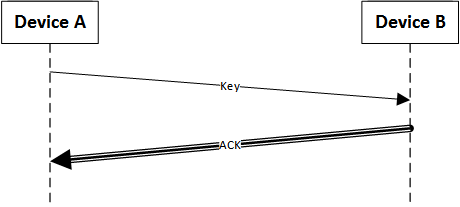
\includegraphics[scale=0.75]{fig/sequence.png}
    \caption{Sequence diagram}
\end{figure}

This authentication scheme requires both devices to have a microphone and a speaker.
The devices must be within close proximity of one another in order to receive the low frequency transmission, which is how the protocol guarantees the secrecy of the symmetric key. If the attacker wants to listen in on the exchange and intercept the key exchange, the attacker must get physically very close to both devices.

The low proximity while exchanging the symmetric key is also the downside of the solution, since both parties who wish to be paired need to be right next to each other.

The solution is also limited in the sense that it requires both devices to have both a microphone and a speaker. One can easily imagine a scenario where this is not the case, such as trying to pair a smartphone with home Hi-fi equipment which propably does not have a microphone. In addition the speakers and microphone on each device must respectively be able to distinguish between 100 different transmitted sounds as well as be able to transmit 100 different sounds, in order for the base-100 encoding to work.

The solution is vulnerable to tampering or interference if an attacker transmits a lot of noise in the same frequency, it would be possible to ruin the key exchange if timed correctly. The key exchange could similarly be ruined if the physical location of the two devices happens to have a lot of ambient noise in the same frequency range.

One possible solution to this problem is to choose a random communication frequency from a pre-defined set of frequencies. A sophisticated attacker might still be able to transmit in all of these frequencies in order to ruin the transmission, but switching frequencies would probably solve the problem of random ambient noise.

Our method has higher hardware requirements than JW, but it provides protection against most common attacks, what JW cannot do. Where JW ask close to none hardware requirements, for our method to work device A has to have speakers and device B has to have a microphone. These hardware requirements are considered low compared to other commonly use pairing methods. Considering security, our method has some weaknesses, but they are hard to exploit. All that makes our method a candidate to replace JW in many devices.

\subsubsection{Solution overview}
\label{subs:Solution overview}
The following activity diagram overviews proposed solution's workflow when no failures occur.

\begin{figure}[h!]
    \centering
    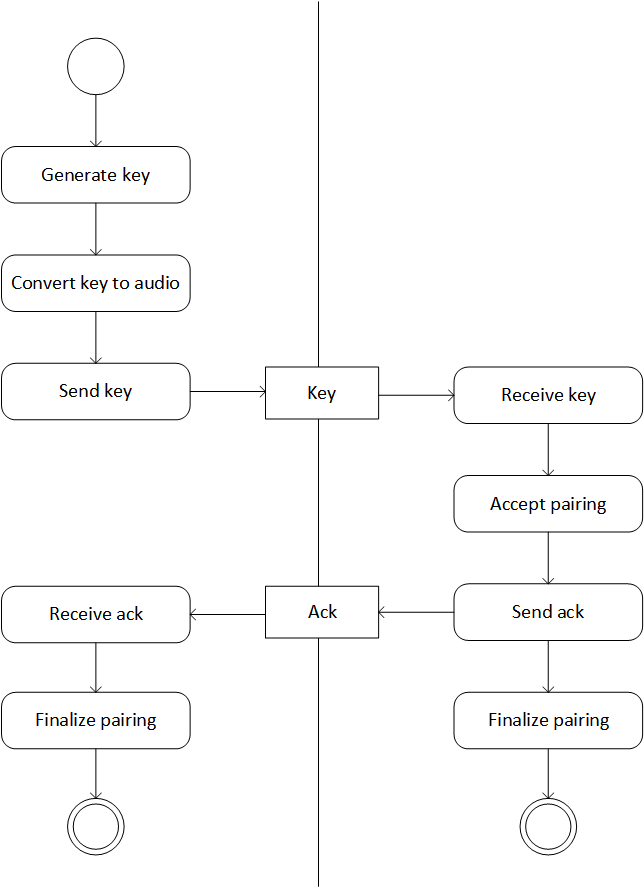
\includegraphics[scale=0.75]{fig/Activities.png}
    \caption{Activities diagram}
\end{figure}

\newpage

The pairing start the pairing device B must be ready to accept the key. Device A initiates the pairing. It starts by generating a random key using pseudorandom number generator. After key is ready, device A converts it to audio by using base-100 encoding and sends to device B through audio channel.
Device B receives transmission sent by device A and by looking for start sequence and end sequence is able to distinguish the key. It stores the key for further communication and sends an acknowledgement to the device A protected using the new key.
Device A knows that pairing was successful if it receives an acknowledgement protected with the sent key.

\subsection{Strengths}
\label{sub:Strengths}

The apparent advantage of using an OOB channel is the fact that it is quite a rare form of communication between mobile devices. This means that a potential intruder will either have to have a wide variety of attacks available, in order to quickly adapt to the sudden use of an obscure OOB channel, or have prior knowledge of the device pairing method being used during device pairing.

Even if the intruder are ready for this specific device pairing method, the fact that the method uses audio during the authentication, makes it extremely difficult for the intruder to temper with the messages being transmitted. This is because sound waves can't be stopped or interrupted, which means the intruder won't be able to change the message, ensuring that correct message will always be sent, thus ensuring authentic communication. Furthermore, we take advantage of the fact, that using low volume audio (With low volume, we mean a low enough decibel, that the devices won't be able to hear the sound outside of a few meters) means that the pairing devices must be close to one another, which means that the intruder must get really close to the pairing, can be difficult.

In addition to the security advantages, utilizing audio for device pairing means that the method will be highly backwards compatible, as almost all, if not all mobile devices (phones) has some kind of microphone and speaker. This further ensures, that the method won't be prone to aging quite as fast as other device pairing methods might.


\subsection{Weaknesses}
\label{sub:Weaknesses}

While our proposed solution has strong authentication, it also has disadvantages, that may prove to be difficult to address. While using audio ensures broad device support, it also relies on the device to be able to record and understand the transmitted messages, which might prove difficult for older devices, where the speaker or microphone might be of poor quality. This is very problematic, as our method won't be able to securely authenticate the devices if the audio can't be understood by the device.

The fact that we use low volume audio to ensure better security also comes with the downside of lessened convenience because the low volume decreases the distance within the devices are capable of pairing.

A potential intruder might have difficulties with tempering with the audio messages sent during authentication, but it is extremely easy to interfere with the pairing in such a way, that the authentication process simply can not be completed. This can be done by broadcasting noise in the same frequency as the authentication messages, which will render the pairing devices unable to understand any message being sent to them.


\subsection{Threat analysis}
\label{sub:Threat analysis}

While we attempt to minimize the ways to compromise our device pairing method, there are still attacks that are hard to deal with, with our chosen method. Our method relies on transmitting a symmetric key in more or less unencrypted form. Because of this, the transmission is prone to eavesdropping, where an intruder may listen to the transmission and get hold of the symmetric key, which means that the intruder will be able to decrypt any future messages between the two paired devices. Additionally, if the intruder gets the symmetric key, it may be possible to also send fake messages to either device, acting as a Man-in-the-middle. We have minimized this risk by utilizing audio as an OOB channel as explained prior, but even if the risk is minimal, it is still there.

Even if the intruder can't get hold of the symmetric key, there are still ways of interfering with the communication of the paired devices. During the authentication of the device pairing, the method relies on transmitting the symmetric key using audio at some inaudible frequency. Because we use audio, the receiving device has to clearly hear the the message, or it may not be able to decode it correctly. The attacker may take advantage of this and broadcast random noise in the same frequency that the device pairing uses. This way, the transmitted message will be obscured, and the receiving device won't be able to decode it, thus preventing the pairing.

\section{Solution analysis}

\subsection{OOB channel}

Much like traditional channels such as WiFi, an OOB channel can be used in the same way to transmit data between devices. However, Out-of-Band (OOB) describes activities outside of defined telecommunication frequency bands. The advantage of using an OOB channel is that it is very uncommon, and thus attackers will have a much harder time making an attack in a given OOB channel. Given a secure protocol, using an OOB channel is not any more secure than a traditional channel. However, for scenarios, where it is not possible to use a sufficiently secure protocol, the protocol can become as secure as the OOB channel.

\subsection{Base-100 encoding}

We require the authenticating devices to be able to either transmit or receive 100 different sounds. This requirement allows us to treat the sounds as symbols in an alphabet with 100 distinct symbols. Such an alphabet would allow us to perform base-100 encoding of the symmetric key, meaning that we essentially can transmit a 256-bit key using only 10 sounds.

An example of this would be the following 256-bit key:

\seqsplit{01010101010010111110000000001010110000010101010101001011111000000000101011000001010101010100101111100000000010101100000101010101010010111110000000001010110000010101010101001011111000000000101011000001010101010100101111100000000010101100000100101011000001}

Which can be encoded into base 100 as \seqsplit{3:7:31:26:22:66:37:53:6:8}.

\subsection{Audio channel}

\subsubsection{The inaudible frequencies}
\label{subs:The inaudible frequencies}

As with electromagnetic spectrum, there is a wide spectrum of audio which humans cannot hear both in frequencies higher than our capacity and in frequencies lower than our capacity. Since higher-frequency audio requires more energy we expect our solution would have better battery performance by using low-frequency audio transmissions.

\subsubsection{Payload structure}
Every time a device wants to share a secret key, it sends the key in the following format:

\begin{itemize}
    \item Start sequence - part where the listening device gets synchronized.
    \item Key sequence - the secret key.
    \item End sequence - end of communication.
\end{itemize}

\begin{figure}[h!]
    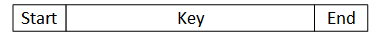
\includegraphics[scale=1]{fig/payload.png}
    \caption{Payload diagram}
\end{figure}


\section{Comparison with state of the art}
\label{sec:Comparison with state of the art}

\subsection{Image scanning}
\label{sub:Image scanning}

Bluetooth SSP using barcode or any other image as Out of Band (OOB) channel is a common practice. The method is as secure as the OOB channel it uses and image scanning as an OOB is very secure. MIDM attacks are practically impossible. The attacker would have to be in very close proximity, few centimeter from the device that generated the image, for a fast interception of the key. Theoretically, if the attacker would have very high quality camera and could get a good angle, it would be possible to capture the image from a greater distance. However, the timeframe to do that is very small as well. The user will scan the code himself/herself quite fast, few second. To do that, he/she will place second device in from of the displayed image, that way shielding it from the attacker. Eavesdropping attacks faces the same problem as MIDM attacks.
Image capture is very secure as an Out of Band channel. However, for this method to work both devices have to have comparably expensive hardware, a camera and a display screen, which is not common in many Bluetooth capable devices. Compared to our solution, we offer a method, which is as secure as image capture method if not even more secure and which could be used by many more Bluetooth devices without having to upgrade the hardware.

\subsection{NFC}
\label{sub:Image scanning}

Using NFC OOB channel for Bluetooth communication is not a common practice, though it is a secure method, secure enough for bank to use it. The NFC works in very close proximity, which gives additional security against MITM and eavesdropping attacks on top of the implemented communication protocols. The reason that it is not used widely for Bluetooth devices pairing is that it is quite new method. Therefore, older devices or the ones which go for a lower price do not have required hardware.

\subsection{Bluetooth 4.0 JW}
\label{sub:Bluetooth 4.0 JW}

JW method is the most commonly used Bluetooth pairing method. It is simple and has low hardware requirements. However, it has no protection against MITM attacks, where our solution provides protection against MITM and does not have high hardware requirements.

\newpage

\section{Conclusion}
\label{sec:Conclusion}

When pairing two devices without the existence of a trusted third party, one can achieve approximately the same guarantee of privacy by using an out of band channel for exchanging encryption keys, assuming that this channel makes it difficult for an attacker to listen on the transmission.

Specifically in the case of inaudible audio as an out of band channel for exchanging keys, we found that it would be very difficult for an attacker to intercept a key exchange, and impossible to reliably modify the communication. Using inaudible audio has the added benefit of being low-cost with respect to hardware requirements and battery usage. It could be implemented on a wide range of devices including smart-watches, cars and smart-phones requiring simply that the devices wishing to be paired in combination have both a microphone and a speaker.

\newpage

\pagenumbering{gobble}
\bibliographystyle{plain}
\nocite{*}
\bibliography{literature}

\end{document}
